\chapter{ВВЕДЕНИЕ В ПОНЯТИЕ СОРЕВНОВАНИЙ ПО ЗАЩИТЕ ИНФОРМАЦИИ}
\label{cha:analysis}

\section{История}
\label{cha:analysis:history}

Согласно «Словарю русского языка» C. И. Ожегова, соревнования~--- форма деятельности (работы, игры), при которой участвующие стремятся превзойти друг друга \cite{Ozhegov89}. Стремление добиваться лучших результатов~--- один из определяющих факторов прогресса.

\Abbrev{ICPC}{International Collegiate Programming Contest ""--- Международная студенческая олимпиада по программированию}

Соревнования естественным образом возникают в разных областях человеческой деятельности. В области информационных и компьютерных технологий это начало происходить в конце XX века. Так, в 1970 году в Техасском университете A\&M были проведены соревнования по спортивному программированию, ныне известные как ICPC \cite{AboutICPC}. Командам участников предлагали решить несколько формально определённых задач на языке программирования «Фортран». Организаторы засекали время и принимали решения на перфокартах: призовые места распределялись согласно времени, которое команда потратила на решение.

На сегодняшний день ICPC — масштабное, уважаемое и значимое соревнование, к победе в котором стремятся сотни тысяч студентов технических вузов по всему миру \cite{AboutICPC}. Возникли и другие соревнования по спортивному программированию, например, Всероссийская олимпиада школьников по информатике \cite{ROI}.

Отрасль, образованная соревнованиями по программированию, внесла существенный вклад в развитие науки и техники. Опыт, получаемый во время тренировок и непосредственного участия в соревнованиях, отразился в компьютерных науках (теория алгоритмов, теория оптимизации, численные методы и др.), методиках преподавания связанных с разработкой программного обеспечения дисциплин и проч. В качестве примера можно привести открытую в 2000 году многократным победителем олимпиад по программированию Николаем Дуровым структуру данных, известную как \textit{декартово дерево по неявному ключу} \cite{Durov00} или возникновение в России системы профориентации школьников и студентов на базе компьютерных школ и сборов, воспитавшей не одно поколение программистов и учёных \cite{Netrusova09} \cite{Kraivanova12}.

По мере распространения компьютерных технологий всё актуальнее становился вопрос об их безопасности. В 1980-х стало зарождаться понятие кибербезопасности \cite{InfosecHistory}~--- совокупности методов и практик защиты от атак злоумышленников для компьютеров, серверов, мобильных устройств, электронных систем, сетей и данных. И в этой сфере появились свои соревнования, Capture the Flag.

\Define{Кибербезопасность}{совокупность методов и практик защиты от атак злоумышленников для компьютеров, серверов, мобильных устройств, электронных систем, сетей и данных}

\Abbrev{CTF}{capture the flag ""--- формат соревнований по защите информации «захват флага»}

История CTF началась в 1996 году, когда были проведены соревнования DEF CON CTF в США \cite{defcon}. Они проходили следующим образом: команды участников находились в общей игровой сети. У каждой команды был запущен разработанный организаторами \textit{сервис} — некая сетевая программа, в которой хранились \textit{флаги} — текстовые строки, модель ценных данных. Используя предусмотренные организаторами уязвимости, флаги можно захватить у другой команды и сдать жюри на проверку. Команда, у которой захватили флаг, теряет баллы, поэтому необходимо не только атаковать соперников, но и защищать свой сервис, внедряя меры по предотвращению несанкционированного доступа других участников к базе данных: например, изменив код компонентов сервиса (иными словами, написав для него \textit{патч~--- информацию, предназначенную для автоматизированного внесения определённых изменений в компьютерные файлы, как правило, в программы, с целью изменения их функциональности либо исправления ошибок).}

\Define{Патч}{информация, предназначенная для автоматизированного внесения определённых изменений в компьютерные файлы. Как правило, в программы, с целью изменения их функциональности либо исправления ошибок}

Со временем CTF-соревнования стали массовым явлением. Свои мероприятия проводят такие крупные IT-комании, как «Яндекс» \cite{YaCTF}, «Лаборатория Касперского» \cite{KasperskyCTF} и другие. За хороший результат в них победителям, как правило, вручают крупные денежные призы или приглашают на работу, как это происходит, например, с финалистами Google CTF \cite{GoogleCTF}.

Интерес к CTF-соревнованиям постепенно появился и за пределами США. В апреле 2008 г. команда «Хакердом» на базе Уральского государственного университета им. А. М. Горького провела открытые межвузовские соревнования по защите информации RuCTF-2008. В игре приняло участие 9 команд со всей России \cite{Hackerdom08}. Сегодня RuCTF~--- международные соревнования, в которых принимают участие сильнейшие команды со всей Европы \cite{Hackerdom20}.

Стоит отметить, что, зачастую организаторы соревнований по защите информации выступают в роли игроков~--- и наоборот. Например, прежде чем стать организаторами RuCTF и популяризаторами CTF в России, команда «Хакердом» на протяжении многих лет занимала высокие места в глобальных рейтингах \cite{HackerdomRating}.

Сегодня CTF продолжает набирать популярность. Агрегатор мероприятий ctftime.org содержит в себе сведения более чем о 1300 соревнованиях, прошедших с 2011 года \cite{CTFTimeTotal}. Соревнования всё чаще проводятся в формате многодневных конференций, на которых игроки выступают с докладами и активно обмениваются опытом, к таким относятся:
\begin{enumerate}
  \item DEF CON CTF, Лас-Вегас, США;
  \item PHDays Standoff и PHDays CTF, Москва, Россия;
  \item VolgaCTF, Самара, Россия;
  \item RuCTF, Екатеринбург, Россия и др.
\end{enumerate}

CTF-соревнования зачастую проводятся в рамках крупнейших российских конференций по информационной безопасности. Компания Positive Technologies, например, проводит соревнования The Standoff, отличающиеся масштабами и зрелищностью. Согласно описанию на сайте мероприятия: «Хакеры находят уязвимости в корпоративных и промышленных IT-инфраструктурах, а специалисты по кибербезопасности нарабатывают опыт предотвращения недопустимых событий. Тысячи зрителей. Неожиданные решения. Незабываемые эмоции» \cite{TheStandoff}. Модели инфраструктуры, с которыми взаимодействуют участники The Standoff, построены по аналогии с реальными современными системами, и в совокупности представляют из себя так называемый «умный город» с предприятиями и офисами. На протяжении всего мероприятия статус этих моделей отражается на интерактивном физическом макете (рисунок \ref{fig:standoff-2022}) со зданиями, дымящимися трубами, горящими индикаторами и т.п., который расположен в зрительном зале.

\begin{figure}[h]
  \centering
  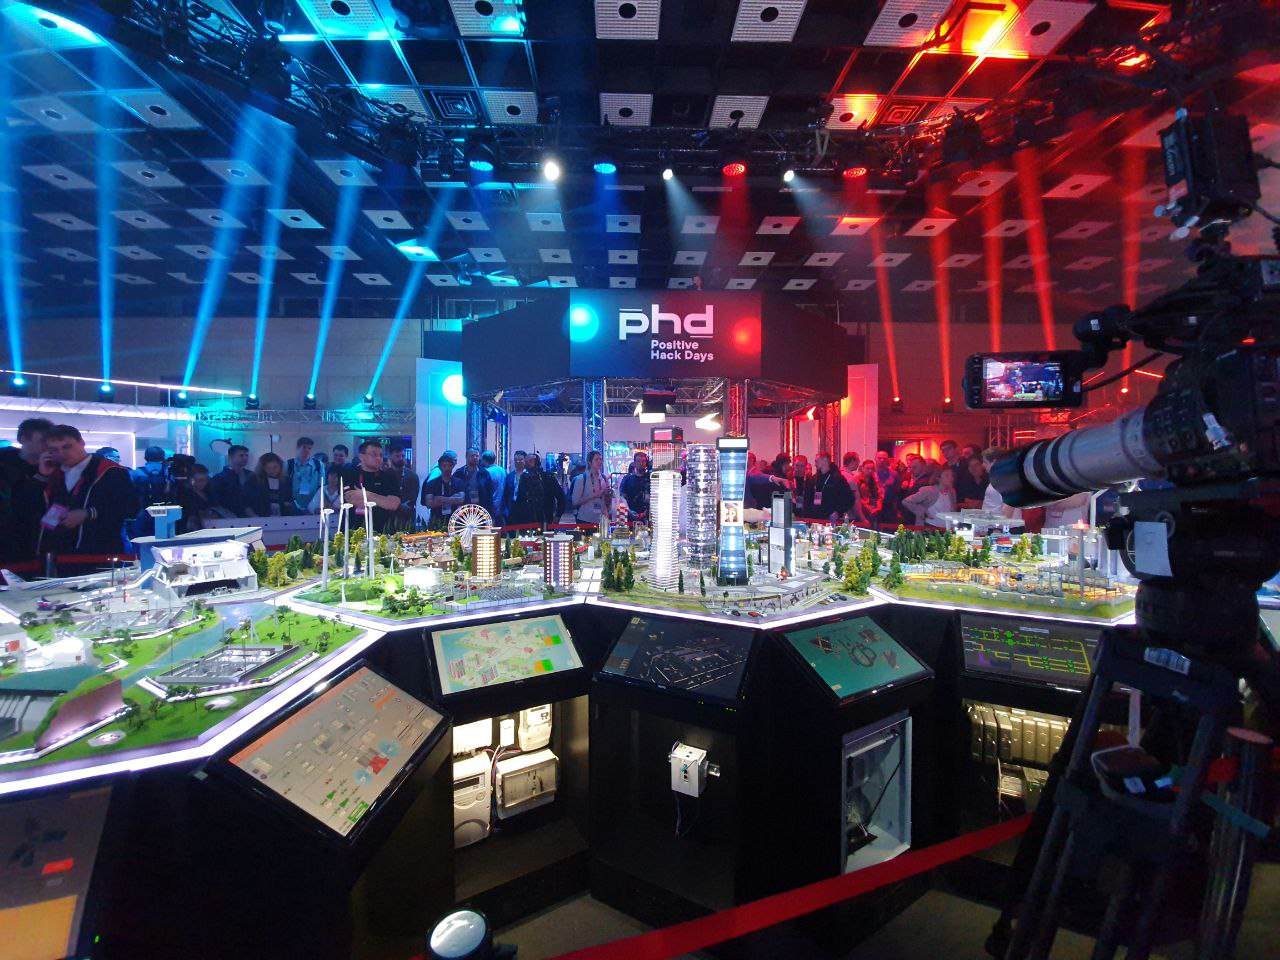
\includegraphics[width=0.6\textwidth]{inc/img/standoff-2022}
  \caption{Макет «умного города» на The Standoff 2022, Центр Мировой Торговли, Москва.}
  \label{fig:standoff-2022}
\end{figure}

Проводятся и образовательные соревнования, нацеленные, не только на студентов и профессионалов в области кибербезопасности, но и на школьников. Важность обучения последних азам защиты информации в теории и практике подтверждается государственным интересом в этой области. В 2017 году министр образования Российской Федерации Ольга Васильева предложила добавить в школьную программу уроки кибербезопасности \cite{RG17}, а с 2018 года по профилю «Информационная безопасность» в формате CTF проводится Олимпиада Национальной технологической инициативы, организации, которая ставит своей целью достижение глобального технологического лидерства России к 2035 году. Автор этой ВКР участвует в разработке и проведении всероссийской школьной олимпиады по защите информации Ugra CTF (см. пункт \ref{cha:analysis:ugractf}).



\section{Правила, принципы и виды}
\label{cha:analysis:rules}

Как отмечалось в \cite{CTFTimeTotal}, за 26 лет истории CTF было проведено как минимум более тысячи мероприятий. Формат CTF нередко подвергался переосмыслению: организаторы продолжают изобретать новые наборы правил, формровать новые системы подсчёта очков, экспериментировать с продолжительностью и масштабностью соревнований.

Неизменным остаётся общий принцип для участников: захватывать флаги. То есть, эксплуатировать предоставленные организаторами уязвимости, чтобы получать доступ к недостаточно защищённой ценной информации.

Появились и разные виды соревнований. Так, вид соревнований, описанный в \ref{cha:analysis:history}, вскоре получил название \textit{Attack-defense (A/D) CTF, (англ. нападение и защита).} Помимо него, выделяют также т.н. Jeopardy CTF \textit{(англ. название телепередачи, известной в России как «Своя игра»)}. Эти виды соревнований различаются правилами, темпом и сложностью игры. Рассмотрим каждый из них отдельно.


\subsection{Attack-defense CTF}

Этот вид соревнований возник первым. К нему относятся, например:
\begin{enumerate}
\item все DEF CON CTF, проведённые с 1996 года по настоящее время;
\item RuCTF;
\item Финальный тур «Кубка CTF России» и др.
\end{enumerate}

Общие положения:
\begin{enumerate}
  \item Соревнования проходят в общей игровой сети (пример структуры такой сети на рис. \ref{fig:ad}). Каждая команда участников имеет в ней собственный сервер, доступный внутри этой сети и называемый \textit{вулнбоксом} \textit{(англ. vulnerable box, дословно «уязвимая коробка»)}.
  \item Участники получают от организаторов набор сервисов — специально разработанного программного обеспечения, имеющего сетевой интерфейс. Нередко этот набор состоит из исходных текстов, которые необходимо скомпилировать и запустить.
  \item Каждый сервис из набора содержит некоторые уязвимости, позволяющие получать несанкционированный доступ к информации, которая в нём хранится.
  \item Командам выдаётся время на подготовку. Сеть в этот момент сконфигурирована таким образом, что каждой команде доступен только собственный вулнбокс.
  \item С окончанием подготовки открывается сеть и начинается игра: включается связь между вулнбоксами разных команд, одновременно с этим начинается отсчёт раундов (как правило, один рануд длится одну минуту).
  \item В течение каждого раунда жюри осуществляет контроль целостности и доступности каждого сервиса каждой команды:
    \begin{enumerate}
    \item пытается осуществить доступ к сервису;
    \item записывает в него один флаг — случайно сгенерированную криптографическим методом строку;
    \item начиная со второго раунда проверяет записанные ранее флаги, сравнивая их с эталонными значениями.
    \end{enumerate}
  \item Нарушить конфиденциальность флагов команды могут только соперники. Они захватывают флаги, используя возможные уязвимости, и сдают их на проверку жюри, получая за это баллы в случае успеха.
  \item Участники вправе исправлять уязвимости в своей системе.
\end{enumerate}

\begin{figure}[h]
  \centering
  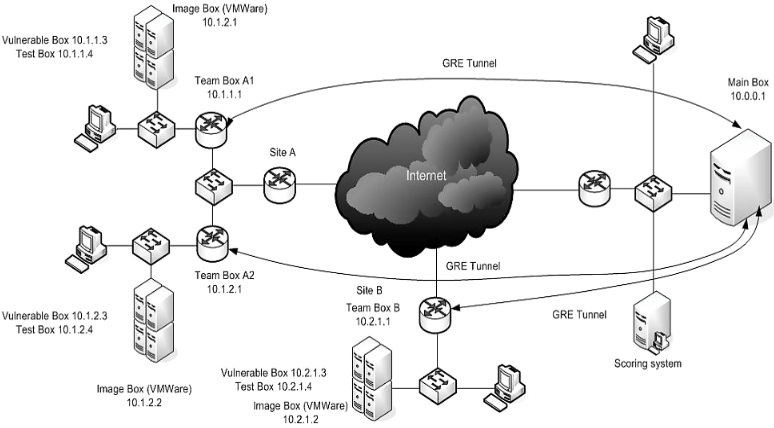
\includegraphics[width=0.9\textwidth]{inc/img/ad}
  \caption{Схема игровой сети UCSB CTF.}
  \label{fig:ad}
\end{figure}

Примерная продолжительность такой игры~--- от пяти до двенадцати часов. Победителей определяют по сумме баллов, набранных за всю игру.

Attack-defense CTF — техничные и требовательные к участникам соревнования. От участников ожидается применение в стрессовой обстановке следующих знаний, навыков и умений:
\begin{enumerate}
  \item серверное администрирование для настройки и запуска игровых сервисов и конфигурации вулнбоксов;
  \item сетевые технологии для понимания поверхности атак, связанных с протоколами, а также для того, чтобы перехватывать трафик (одна из стратегий игры~--- наблюдать, как другие команды эксплуатируют уязвимости и как можно быстрее повторять их действия \cite{ReplayAttacks});
  \item чтение программного кода сервисов, который может быть написан на любом языке программирования; и т.п.
\end{enumerate}



\subsection{Jeopardy CTF}
\label{cha:analysis:Jeopardy}

Jeopardy CTF — второй распространённый вид соревнований. В нём участники соревнуются в решении задач на время \cite{Course}.

Своё название данный вид соревнований получил благодаря схожести с форматом телепередачи «Своя игра», в которой игроки выбирают вопросы, сгруппированные по темам и стоимости, с той лишь разницей, что в CTF команды решают задачи асинхронно и не должны видеть решения других команд. Таким образом, соревнования вида Jeopardy больше похожи на соревнования по спортивному программированию, где участники получают баллы за верно решённые формально описанные задачи и дисквалифицируются за нечестную игру: списывание или получение иной внешней помощи.

Общие положения:

\begin{enumerate}
  \item Участникам предлагается одинаковый набор задач \textit{(англ. challenges)}.
  \item Участникам о каждом задании известны его:категория, стоимость (баллы, которые принесёт верное решение) и текстовое услови.
  \item В ходе решения задачи участники получают флаг — текстовую строку заранее известного формата, которую можно сдать жюри на проверку. Верный флаг означает, что задача решена успешно.
  \item В конце соревнований подводят итоги. Побеждают участники, набравшие наибольшую сумму баллов к концу соревнований. В случае равенства выше оцениваются те, кто раньше сдал последний флаг.
\end{enumerate}

\Define{Метаданные}{\textit{(от греч., дословно: «данные о данных»)} — дополнительная сопровождающая информация, как правила обладающая хорошо выраженной структурой.}

\begin{figure}[h]
  \centering
  \includegraphics[width=0.8\textwidth]{inc/img/Jeopardy}
  \caption{Главная страница игровой системы Ugra CTF.}
  \label{fig:Jeopardy}
\end{figure}

На Jeopardy CTF разрешается пользоваться интернетом и справочной литературой, поскольку решение задач может требовать от участников способности оперативно разобраться в новой, незнакомой теме или конкретной технологии. Встречаются задачи, например, на:
\begin{enumerate}
\item определение места съёмки фотографии по виду из окон \cite{BigcitylightsTask},
\item реверс-инжиниринг сложных обфусцированных программ, написанных на малопопулярных языках \cite{ReverseTask},
\item на традиционный поиск уявзимостей в программах \cite{WebTask} и т.п.
\end{enumerate}

Несмотря на такое разнообразие материала, в Jeopardy CTF возникла устойчивая классификация задач по категориям, которую используют подавляющее большинство организаторов и участников (усреднённый перечень наиоболее распространённых категорий дан в таблице \ref{tab:categories}). Это объясняется тем, что грамотно составленные метаданные задачи позволяют игрокам быстро определять их сложность и эффективно распределять свои силы в условиях ограниченного времени.

\begin{longtable}{|p{0.12\textwidth}|p{0.82\textwidth}|}
    \caption{Некоторые категории CTF-задач.}
    \label{tab:categories}
    \\ \hline
    \textbf{Название} & \textbf{Пояснение}
    \\ \hline \endhead
    \texttt{crypto}   & Криптография: задачи о слабых криптоалгоритмах \\
    \texttt{stegano}  & Стеганография: искусство тайной передачи информации \\
    \texttt{osint}    & Разведка по открытым источникам: поиск информации в интернете \\
    \texttt{ppc}      & Программирование: автоматизация \\
    \texttt{reverse}  & Реверс-инжиниринг: анализ бинарных файлов или работы программ \\
    \texttt{web}      & Веб-технологии: браузерные и серверные уязвимости \\
    \texttt{network}  & Компьютерные сети \\
    \texttt{admin}    & Администрирование: знание ОС и ПО \\
    \texttt{hardware} & Аппаратные устройства: микроконтроллеры, электротехника и т.п. \\
    \hline
\end{longtable}

\Abbrev{ОС}{Операционная система}
\Abbrev{ПО}{Программное обеспечение}

Данная работа посвящена разработке среды для проведения соревнований по защите информации именно этого вида.




\section{Соревнования по защите информации Ugra CTF}
\label{cha:analysis:ugractf}

На момент написания данной ВКР автор проходит практику в Югорском научно-исследовательском институте информационных технологий. При поддержке этого института, а также по инициативе Департамента информационных технологий и цифрового развития Ханты-Мансийского автономного округа — Югры, в России с 2016 проводятся соревнования по защите информации Ugra CTF.

Олимпиада проводится с целями выявления и работы с талантливой молодёжью, а также для профессиональной ориентации обучающихся на деятельность в сфере информационной безопасности \cite{Olymp}. Ugra CTF — значимое мероприятие международного масштаба:

\begin{itemize}
\item
  вокруг олимпиады построена основная профориентационная площадка в области кибербезопасности и информационных технологий для школьников Югры и других регионов страны;
\item
  заключительные этапы соревнований в 2016---2019 годах проходили при международном IT-форуме с участием стран БРИКС и ШОС в городе Ханты-Мансийске;
\item
  параллельно с отборочным этапом олимпиады проходит неофициальный зачёт для всех желающих, стабильно привлекающий большое количество участников, в том числе из-за рубежа: в 2022 году в нём приняло участие более 900 человек из стран СНГ, Индии, Китая, Великобритании, США и других стран.
\item
  победители и призёры соревнований из года в год поступают в ведущие вузы России по профильным направлениям, успешно участвуют во всероссийских и международных соревнованиях.
\end{itemize}

Традиционно соревнования Ugra CTF проводились в два этапа: дистанционный отборочный для всех желающих и очный заключительный (финал) для лучших игроков, проводившийся в столице ХМАО, Ханты-Мансийске. Как правило, оба этапа представляли собой CTF вида Jeopardy.

\begin{figure}[h]
  \centering
  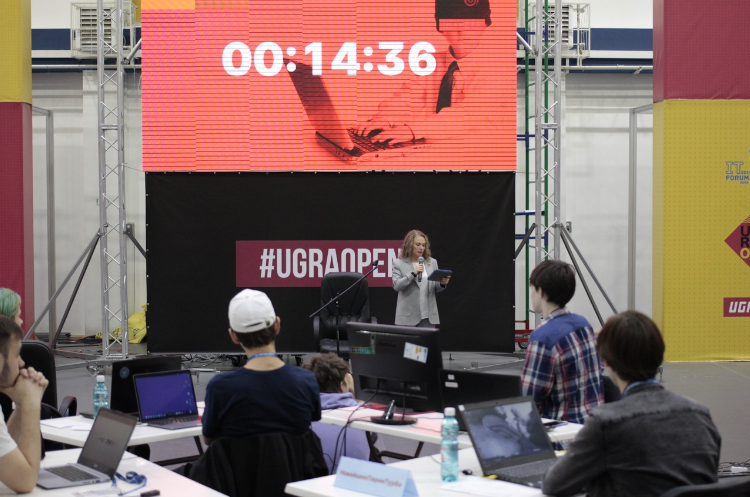
\includegraphics[width=0.8\textwidth]{inc/img/ugractf-19}
  \caption{Открытие Ugra CTF Finals 2019. 10 июня 2020 года, Ханты-Мансийск.}
  \label{fig:ugractf-19}
\end{figure}

\Abbrev{ХМАО-Югра}{Ханты-Мансийский автономный округ — Югра}

В 2019–2020 году в состав организаторов вошёл Департамент образования и молодежной политики ХМАО-Югры. Примерно в это же время в России стало наблюдаться снижение числа регулярных CTF-соревнований для школьников: по разным причинам прекратили свою деятельность организаторы соревнований UfoCTF и QCTF \cite{QCTF}, основных российских соревнований для новичков.

В связи с этим, были внесены изменения в схему проведения соревнований — для школьников с 2021 года проводится отдельный \textit{распределённо-очный} индивидуальный заключительный этап по правилам Российского совета олимпиад школьников с перспективой получения официального статуса и внесения Ugra CTF в перечень олимпиад Российского совета олимпиад школьников \cite{Rosolymp}. Это позволит победителям получать привилегии при поступлении в высшие учебные заведения.

В отборочном этапе 2021 года приняли участие 233 школьника в составе 93 команд. Помимо этого, более 450 команд со всего мира выполняли задания олимпиады в неофициальном зачёте \cite{UgraCTF}. В том же этапе, но в 2022 году, приянло участие уже 383 школьника из 159 команд. Из них более ста человек прошли в финал.

Для того, чтобы все финалисты смогли принять участие, команде разработки необходимо предоставить несколько десятков особым образом настроенных рабочих станций: от Санкт-Петербурга до Владивостока, и обеспечить бесперебойность работы всей инфраструктуры соревнований.


\section{Распределённо-очный формат проведения CTF-соревнований}
\label{cha:analysis:}

\Abbrev{РСОШ}{Российский совет олимпиад школьников}

Распределённо-очный заключительный этап~--- компромисс между:
\begin{enumerate}
  \item полностью дистанционным проведением олимпиады, запрещённым правилами РСОШ ввиду отсутствия возможности контролировать участинков;
  \item полностью очным проведением, когда все участники собираются на единой площадке, полностью контролируемой оргкомитетом.
\end{enumerate}

При таком формате соревнования проходят в разных городах на разных площадках, предоставляемых партнёрами оргкомитета: частными фирмами, образовательными организациями или муниципалитетами.
Сотрудники этих организаций на период проведения олимпиады выступают в роли наблюдателей, в обязанности которых входит инструктаж участников, подготовка рабочих мест и контроль за соблюдением регламента олимпиады на протяжении всего мероприятия.

При распределённо-очном проведении соревнований существенно повышается охват участников: дети более склонны принять участие в олимпиаде, если для этого не нужно ехать в другой город. Однако, проводить такую олимпиаду на порядок сложнее. Это можно объяснить целым рядом причин.

Во-первых, при таком подходе не всегда возможно очное взаимодействие организаторов, наблюдателей и участников. Участников оргкомитета меньше, чем городов, в которых на данных момент проводится Ugra CTF. Вместо того, чтобы пытаться быть везде одновременно, команда разработки тщательно отлаживает протоколы взаимодействия с площадками, создаёт инструкции и регламенты и централизованно контроллирует ход игры на всех этапах из единого штаба.

Во-вторых, необходимо свести к минимуму факторы, влияющие на неравенство участников: ситуации, в которых участники на разных площадках решают тур олимпиады в разных условиях недопустимы. Соревнования должны начаться и закончиться одновременно, любые технические неполадки должны оперативно исправляться, а наблюдатели должны строго соблюдать регламент проведения олимпиады и правила РСОШ.

В-третьих, соревнования по кибербезопасности в формате CTF требовательны с технической точки зрения. Программное и аппаратногое оснащение рабочих станций участников является решающим фактором при участии в олимпиаде. Зачастую требуются привилегированный доступ к системе и специализированные программные инструменты; к тому же дополнительные трудности могут возникать и в свете того, что многие игроки предпочитают использовать UNIX-подобные операционные системы. Соответствующим образом настроить инфраструктуру в нескольких местах по всей стране в ограниченные сроки, учитывая разный уровень технической квалификации наблюдателей — непростая задача.

Так же непросто обеспечить гарантированное соблюдеине порой неочевидных правил проведения соревнований. Например, согласно правилам РСОШ переговоры участников и получение внешней помощи запрещены, однако, ввиду специфики соревнований пользоваться интернетом школьникам разрешается. Возникает закономерный вопрос: как отличить легитимное использование сети от тщательно замаскированной попытки опубликовать решение и получить помощь третьего лица?

Наконец, участникам — и только им — необходимо иметь беспрепятственный доступ к материалам олимпиады — непосредственно, CTF-задачам. Распространять и публиковать условия, а также обсуждать решения задач запрещено на протяжении всего мероприятия, притом материалы должны быть доступны всем участникам единовременно.

Таким образом, возникает необходимость в разработке системы, которая бы:
\begin{itemize}
\item
  обеспечивала контроль решения материалов олимпиады участниками (включая выдачу условий, проверку решений и подведение итогов);
\item
  позволяла оргкомитету выявлять факты нарушения правил и регламента как участниками, так и наблюдателями (включая задержки, общение участников и т.п.);
\item
  предоставляла участникам комфортную среду для решения задач с учётом высоких системных требований, накладываемых спецификой формата CTF,
\item
  легко масштабировалась на любое число площадок и любую вариацию условий (часовые пояса, качество подключения к интернету).
\end{itemize}

\section{Выводы}

CTF-соревнования — современный и эффективный способ оценки знаний, навыков и умений в сфере кибер- и информационной безопасности, позволяющий осуществлять такую оценку в игровом формате. Проведение CTF-соревнований — актуальная и значимая тема, о чём говорит большое число международных соревнований, признание формата CTF на государственном уровне в сфере российского образования и общая важность вопросов информационной безопасности.

В России проводятся соревнования Ugra CTF, к разработке которых причастен автор данной работы. С 2021 года оргкомитет соревнований проводит CTF-соревнования для школьников в распределённо-очном формате по правилам Российского совета олимпиад школьников. Организация подобных мероприятий в масштабе всей страны — серьёзная и непростая задача, решение которой предоставляет широкий простор для оптимизации с учётом большого количества требований, которым необходимо удовлетворять.

Детально рассмотрев организационно-технический процесс по подготовке и проведению олимпиады, можно выделить в нём и оценить подлежащие автоматизации этапы.



%%% Local Variables:
%%% mode: latex
%%% TeX-master: "rpz"
%%% End:
